\documentclass[portfolio.tex]{subfiles}
\begin{document}
	\Chapter{Week 6}{Data Binding}
	\section{Weekly Content}

			\section{Introduction}
				This week adds another useful tool into our Vue repertoire - Two-Way Binding. This combines two concepts from the previous week, \textbf{props} and \textbf{events}. This is another great way to reduce the amount of code we have to write. \\

				In a theoretical sense, two-way binding one of the direct implementations of the Model-View patterns we studied last week as well.\\

			\hspace{-0.6cm}
			\splitpage{
			\subsection{Two-Way Binding}
			Data binding describes how data is passed between the model and the view. One-Way binding means that data only travels one way. For example, data in the model, can be passed to the view, but the view cannot update data in the model.  In Vue, this would be the v-bind directive and props, where information is only passed from the parent to the child.\\

			Two-way binding on the other hand is bi-directional. That means as before, the data passes from the model to the view, but now the view can directly update the data in the model. In Vue, this is the v-model directive. An input field takes in a value from the parent, and then returns any updates. This means that the source of truth lies solely in the parent component.\\
			}{
				\centering
				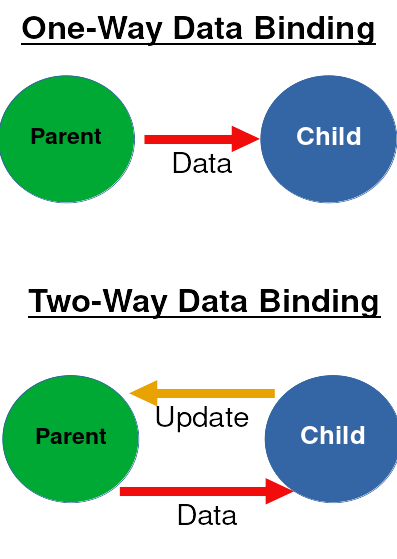
\includegraphics[width=0.8\linewidth]{Data Binding.png}
			}

			\vspace{0.5cm}

			v-model can be manually implemented as well. Depending on the input type, different directives can be used. For example input would use v-bind:value to pass the value to the input, and then v-on:input event to update the value whenever the input changes.\\

	\section{Individually Researched Topics}
		\subsection{Introduction}
			In addition to the concepts discussed in the class, I was curious about more advanced topics within Vue, and how they could improve my project. The main features I added to my project were Vue Router, Vuex, Composition API and Vue Transitions.

		\subsection{Vue Router}
			\textit{As I was programming my project, I was wondering how to link up my different views, and how to choose which one to display. This led me to Vue Router, and trying to understand how it works.}\\

			Vue Router is an easy way to manage url paths within an application. There are three main steps to using Vue Router. \\

			The first is setting up the router. The router can be set up in the main.js, or more cleanly it its own JavaScript file and then imported into main.js. The main options needed when setting up the router is the possible routes, and the history. There are many other available options to configure the routers further. Here is an example router setup:\\

			\begin{lstlisting}
// 1. Define route components.
// These can be imported from other files or for very small components defined directly in the router
import Home from './components/Home';
import NotFound from './components/NotFound';
const About = { template: '<div>About</div>' }

// 2. Define some routes
// Each route should map to a component.
const routes = [
{ path: '/', component: Home },
{ path: '/about', component: About },
// A general path for any unmatched path, which redirects to a not found component.
{ path: '/:pathMatch(.*)', name: 'NotFound', component: NotFound },
]

// 3. Create the router instance and pass the `routes` option
const router = VueRouter.createRouter({
	// 4. Provide the history implementation to use. We are using the hash history for simplicity here.
	history: VueRouter.createWebHashHistory(),
	routes, // short for `routes: routes`
})

// 5. Create and mount the root instance.
const app = Vue.createApp({})

// Tell the app to use the router
app.use(router)

app.mount('#app')
			\end{lstlisting}
		Modified from \autocite{vue-router}.\\

		I set up my router in its own JavaScript file, follow the link to see this: \\
		\seqsplit{https://github.com/BrandonMurch/SIT120/blob/021a2694432d61e32c9fba191ee7579c2dfdb955/Assignment\%201/updated-proof-of-concept/tend/src/router/index.js}\\

		Setting up Vue Router is, by far, the most complicated part. To use Vue router, only two main tags are needed. The first is $<$router-view$>$ which is where the selected component is placed depending on the route, and renders it inside. The other is $<$router-link$>$, which replaces the $<$a$>$ tag, to be able to work seamlessly with Vue Router. The \textbf{to="target"} attribute is used to choose which path to go to on click. \\

		\subsection{Vuex}
			\label{vuex}

			\textit{I also needed a way to store user login information within my application. At first I stored this in the App component. This was very messy and didn't work very well. This caused me to look into Vuex, as a way to centrally store information. }\\

			Vuex is a great way to share information within the entire application. Vuex will create a "store" where information will be stored in one place.\\

			Vuex uses the "State Management Pattern". To understand this pattern, it is useful to first understand the naive approach. This approach is to simply store the data in a variable. If this method is used, any component can access, and \textbf{modify} the data. There is no way to keep track of who has modified the data, if the component has permissions to modify the data, and what modifications are allowed. For example, if there is a "personAge" property in the store, there is no way to prevent a component from changing the variable to "Donkey". \\

			\hspace{-1.4cm}
			\vspace{0.2cm}
			\splitpage{
				\centering
				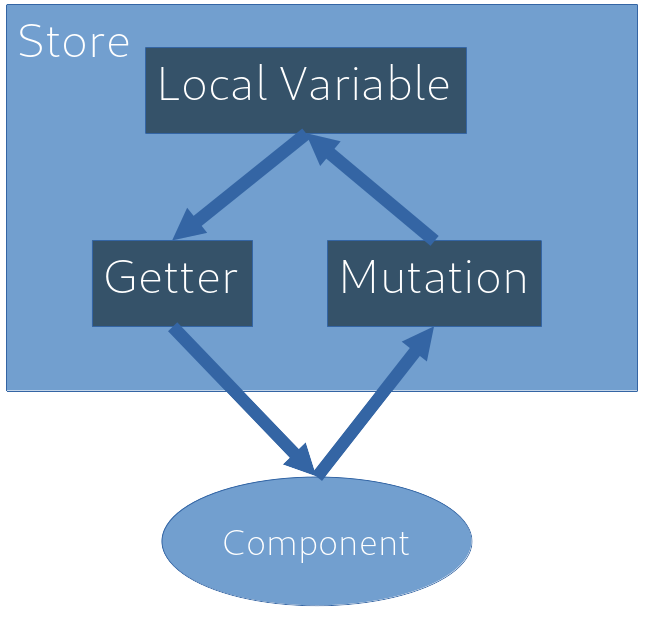
\includegraphics[width=0.8\textwidth]{state-management-pattern.png}
			}{
			The "State Management Pattern" addresses this by not allowing components to directly modify the variable. Instead the pattern creates actions or mutations that can be performed, with certain variables that can be passed in. If a component "commits" one of these mutations, the store is then able to verify the data coming in (making sure it is a number for the previous example), make modifications if necessary, and then place it within the appropriate variable. With this pattern, logs can also be created every time the store is modified. \\}

			To use the store, there are multiple categories of actions that can be defined. Getters are functions that return a value within the store. This could also be a more complicated function, for example within the store could be firstName and lastName, and a getter function could be getFullName, which would concatenate firstName and lastName together. A code example:\\
			\begin{lstlisting}
const getters = {
	username: (state) => {
		console.log(state)
		if (state.isLoggedIn) {
			return state.user.name;
		}
		throw new Error("There is no user logged in.")
	}
}
			\end{lstlisting}
			\bigbreak
			This getter attempts to get the username of the logged in user. If there is no user, it throws and error. \\

			Another category of actions that can be defined are mutations. Mutations are a way of changing the state of the store. This category was provided in the earlier example of setting personAge. A code example:\\

			\begin{lstlisting}
const mutations = {
	logUserIn(state, name) {
		state.isLoggedIn = true;
		state.user.name = name;
	}
}
			\end{lstlisting}
			\bigbreak
			This logs a user in and also sets the isLoggedIn boolean to true;\\


			Actions call mutations. The difference between the two is that mutations are synchronous, while actions can be asynchronous. For example, an action could be an asynchronous call to a server for more information, which then calls a mutation to commit the information once it is loaded. An example from Vue which increments a counter only after 1 second has passed:\\

			\begin{lstlisting}
actions: {
	incrementAsync ({ commit }) {
		setTimeout(() => {
			commit('increment')
		}, 1000)
	}
}
			\end{lstlisting}
			\autocite{vuex}

			\subsubsection{Source Code}
				My Vuex store is located in

		\subsection{Composition API}
			\textit{I was curious about new features within Vue 3, so I began with the largest change, and investigated how I may implement it in my own project.}\\

			With Vue 3, the composition API is a new way to set up components. The Composition API replaces the data function, the methods object  and more, within a component. This allows for two things to happen, first of all this allows for similar concepts to be group together. with the previous API, you might have the following code:\\

			\begin{lstlisting}
export default {
	name: "NavigationBar",
	data() {
		return {
			isMenuOpen: false
			links: [...]
		}
	},
	methods: {
		toggleMenuOpen() {
			...
		}
		addLink() {
			...
		}
	}
}
			\end{lstlisting}

		The problem with this is that there are two separate areas of concern. One that is handling the state of whether the menu is open or not, and the other that is handling which links are being displayed. It would be nice to group these together. This is where the composition API comes in. It allows these different parts of the component to be grouped in on \textbf{setup} function:\\

		\begin{lstlisting}
export default {
	name: "NavigationBar",
	setup() {

	// ======= Handle Open Menu ========
		let isMenuOpen = false;
		toggleMenuOpen() {
			...
		}

	// ======= Handle Links ==========
		const links = [...]
		addLink() {
			...
		}
		return {
			isMenuOpen,
			toggleMenuOpen,
			links,
			addLink,
		}
	},
}
		\end{lstlisting}

		This nicely groups the two areas of concern. This also allows easy separating groups of like variables and functions into separate files, which can then be imported easily. This increases reusability and the clarity of the code.\\

		\autocite{vue-composition}

		\subsection{Vue Transitions}
			\textit{Within my project, I noticed that I was unable to use the standard CSS transitions while using v-if, or v-for. This lead me to look into entering/exiting transitions, as well as list transitions.}\\

			Vue transitions work closely with directives such as v-if, or v-for. Transitions can be used with v-if for example, to add transitions when the component leaves or enters the DOM. This would use the $<$transition$>$ tag as follows:\\

			\begin{lstlisting}
<transition name="fade">
	<MyComponent
	v-if="booleanStatement"
	/>
</transition>
			\end{lstlisting}
		\bigbreak

		The transition can be named anything the user desires. It can even be dynamic. This connects it to a set of style attributes that describe how the transition will look. For the example of this transition named \textbf{fade} the style would look like:\\

		\begin{lstlisting}
.fade-enter-active{
	transition: all 0.5s !important;
}
.fade-leave-active {
	position: absolute;
	transition: all 0.5s;
}

.fade-enter-from,
.fade-leave-to {
	opacity: 0 !important;
}

.fade-enter-to,
.fade-leave-from {
	opacity: 1 !important;
}

		\end{lstlisting}

			\bigbreak
			\noindent
			\textbf{fade-enter-from} and \textbf{fade-leave-to} refer to the states that occur one frame before entering and after leaving. This means that the element will both have a opacity of 0 before and after.\\
			\\
			\textbf{fade-enter-to} and \textbf{fade-leave-from} handle what the element will look like directly after entering or before leaving. \\
			\\
			\textbf{fade-enter-active} and \textbf{fade-leave-active} handle the animations during the transition. Any custom transitions can be created by using the \textbf{\{NAME\}}-enter-from, etc. templates and then placing that \textbf{NAME} in the name attribute of transition.\\

			\begin{center}
				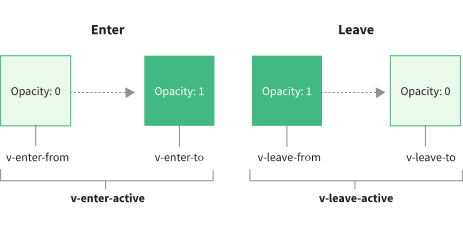
\includegraphics[width=0.8\linewidth]{transitions.png}\\
				\autocite{vue-transitions}
			\end{center}

			Vue Transitions also include a $<$transition-group$>$ tag. This handles the transitions for lists of elements that use v-for to render. This will animate when new elements are added to the list, or removed. transition group uses the same style templates as transition, but adds one more option for \textbf{\{NAME\}-move}, which will add a transition for elements shifting to accommodate new elements. For example, the following will take 0.5 seconds to slide an existing element down/up:\\

			\begin{lstlisting}
.fade-move {
	transition: all 0.5s ease;
}
			\end{lstlisting}

			\vspace{0.5cm}
			It is difficult to display transitions within a screenshot. To get a better idea of how I implemented these transitions, please visit:
			 \begin{center}
				 \Large\seqsplit{tend.brandonmurch.com}.
			 \end{center}


		 \subsection{Deployment}
		 	\textit{I wanted to easily share my design so far. I figured the best way to do this would be on my website. I set out to deploy my application to tend.brandonmurch.com. }\\

		 	Running a VueCLI-based application requires an extra step to deploy. Thankfully this only requires one command to the terminal:

		 	\begin{center}
				\textbf{npm run build}
		 	\end{center}

	 		This will combine all the separate component files, and JavaScript files into one or a few  files, and link them into index.html. This places these JavaScript files, along with the other asset files such as CSS, and images into a \textbf{dist} folder. This folder can then be uploaded to the server of your choice, as if you had written everything in plain HTML/CSS/JavaScript.\\

		 	One difficulty comes when using Vue Router. Since Vue Router wants to handle all the routing, the website must always be directed to the base route first. Since I was deploying this to Netlify, I followed the example on Vue Router's guide and created a file in my public folder called \_redirects, which contained:\\

		 	\begin{lstlisting}
/* /index.html 200
		 	\end{lstlisting}

	 		\bigbreak
	 		This meant that any route should be redirected to index.html, and return the HTTP code 200 OK. This means that when visiting www.website.com/my/long/path. The server will redirect to www.website.com and let Vue Router handle the rest. \autocite{vue-router} \\

	 		Finally, since I was not using the default given URL from Netlify, I had to update a DNS File. This involved creating a CNAME record and pointing it at the default given URL. I followed along with the instructions here: \\

	 		\seqsplit{https://docs.netlify.com/domains-https/custom-domains/configure-external-dns/}\\

	 		Thankfully web hosting services such as Netlify, Github Pages, etc. handle most of the heavy lifting. We don't have to manage things like SSL Certification manually.

	 	\subsection{DNS Records}
	 		\textit{After deployment, I was curious about the different types of DNS records. What is CNAME? What were the instructions I just followed to get this website deployed? Are there other types of DNS records?}\\

	 		\subsubsection{Subdomains}
	 			A subdomain uses the same address as your regular domain, but instead will put additional information \textbf{BEFORE} the domain. For example, if the main domain was website.com, then a subdomain could be blog.website.com which hosts a blog. A different service could be running on store.website.com. This allows for services that are hosted of different servers to be "linked" for the user with a common domain.

	 		\subsubsection{CNAME}
	 			A CNAME record is like a redirect. It points to a different address, which could be another CNAME Record, or an A record. If it points at another CNAME, then a chain will be created. Many CNAME records could be added on to this chain, but it must eventually end with an A record.\\

	 			In this case I was able to use a CNAME record to create a subdomain which pointed at the Netlify. \autocite{cloudflare-CNAME}

	 		\subsubsection{A Record}
	 			\textit{So we know what a CNAME record is, and that it eventually will point to an A record, but what is an A record?}\\

	 			This is the main address of a server. This is what you would normally think about when DNS record is mentioned. That is, a user-readable string which translates directly to an IP address.  \autocite{cloudflare-A}



	\section{Practical Tasks}
		\subsection{Task 1}
			This task was all about the basics of two-way data binding in Vue. I created an input, as well as a local variable and linked them with two way binding.\\

			I used v-model within my contact form in my project.

			\subsubsection{Source Code}
				\seqsplit{https://github.com/BrandonMurch/SIT120/blob/021a2694432d61e32c9fba191ee7579c2dfdb955/Assignment\%201/updated-proof-of-concept/tend/src/components/TheContactForm.vue}

			\subsubsection{Screenshot}
				The form looks like:

				\begin{center}
					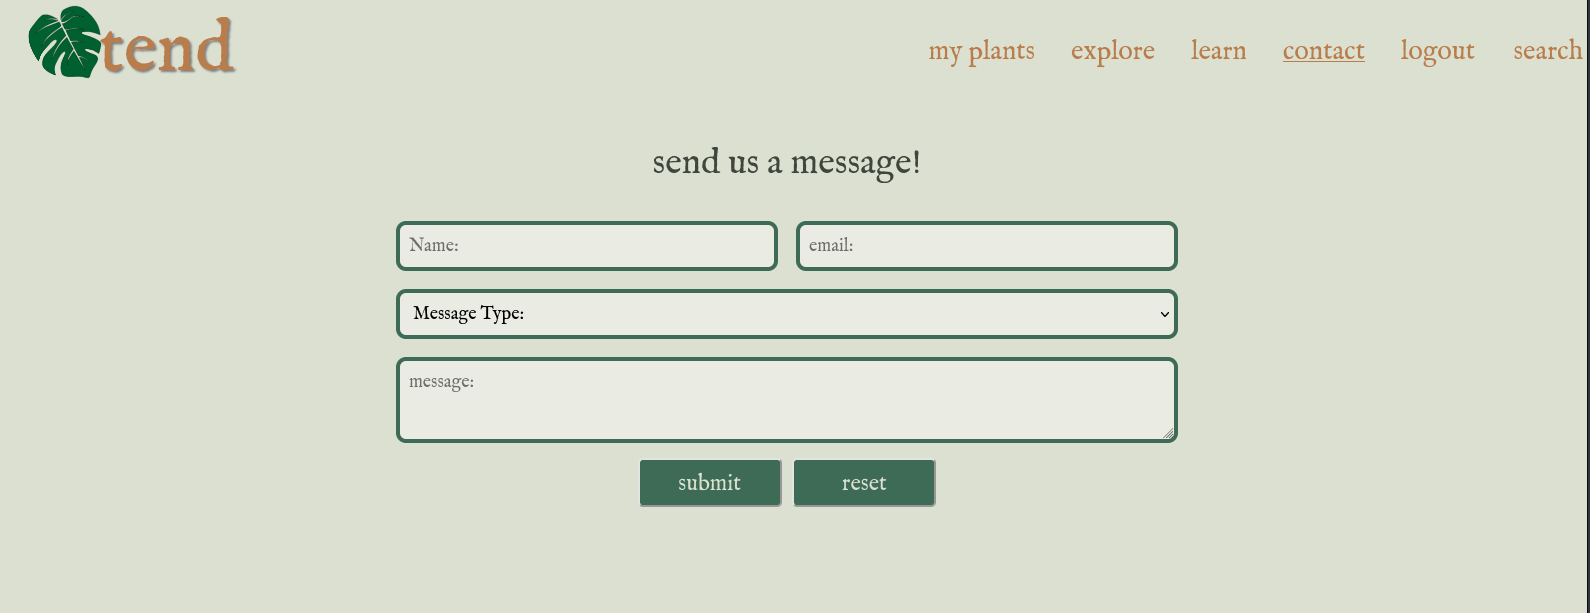
\includegraphics[width = 14cm]{contact form.png}
				\end{center}

				On form submit, a message is presented to the user. The variables within the message are assigned using two way binding.

				\begin{center}
					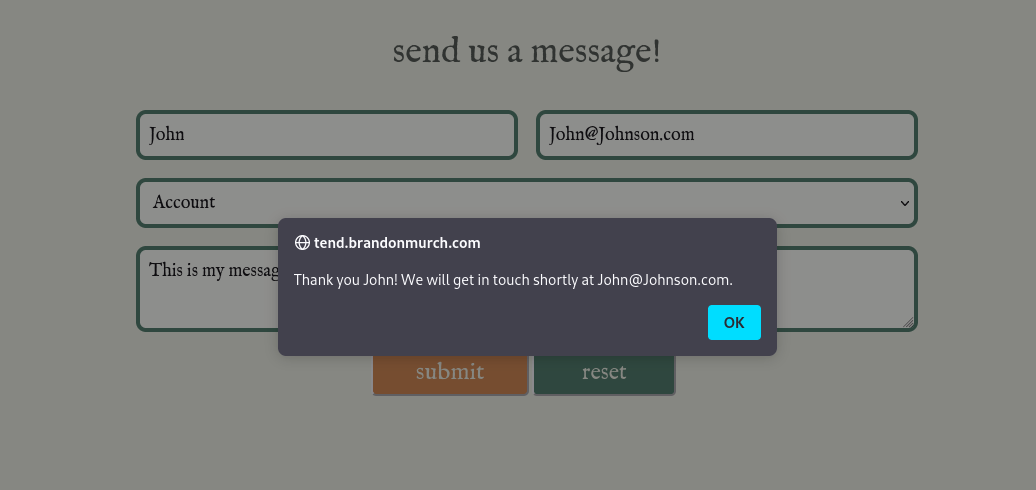
\includegraphics[width = 14cm]{submitted-contact.png}
				\end{center}

		\subsection{Task 2}
			Checkboxes are an important part of a form and can either represent a boolean value, or the ability to choose multiple fixed values.\\

			I used a checkbox within my login form. Clicking it will allow the user to be remembered by the application and not have to login again on that machine. It will contain two-way binding to a rememberMe variable within the user object.

			\subsubsection{Source Code}
				\seqsplit{https://github.com/BrandonMurch/SIT120/blob/021a2694432d61e32c9fba191ee7579c2dfdb955/Assignment\%201/updated-proof-of-concept/tend/src/components/TheLoginForm.vue}
			\subsubsection{Screenshot}
				The form looks like:

				\begin{center}
					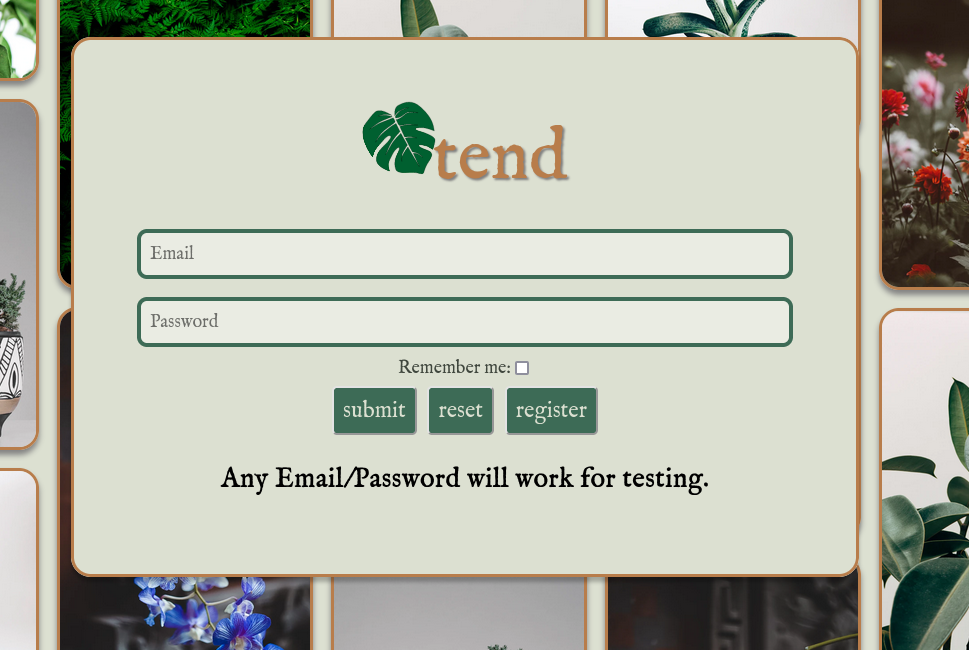
\includegraphics[width = 14cm]{login form.png}
				\end{center}

		\subsection{Task 3}
			Being able to render options dynamically for a select element, saves a lot of repeating code. Instead a list of strings or a list of objects can be passed in.\\

			I used a dynamically rendered options list within my contact form in my project. Users could select the reason they were contacting the company.
			\subsubsection{Source Code}
			\seqsplit{https://github.com/BrandonMurch/SIT120/blob/021a2694432d61e32c9fba191ee7579c2dfdb955/Assignment\%201/updated-proof-of-concept/tend/src/components/TheContactForm.vue}


			\subsubsection{Screenshot}
			The form with the options looks like:

			\begin{center}
				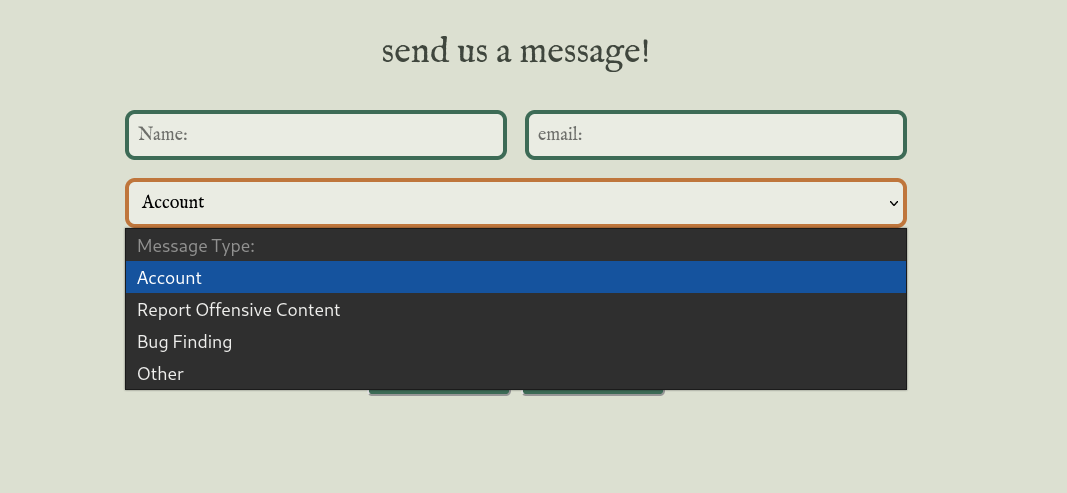
\includegraphics[width = 14cm]{contact-options.png}
			\end{center}

		\subsection{Task 4}
			Modifiers add quick ways to perform common tasks. It saves code, and energy not having to reimplement the same common features over and over.\\

			I used trim within my SearchBar input to remove extra white spaces and make matching entries much easier.

			\subsubsection{Github Link}
				\seqsplit{https://github.com/BrandonMurch/SIT120/blob/021a2694432d61e32c9fba191ee7579c2dfdb955/Assignment\%201/updated-proof-of-concept/tend/src/components/SearchBar.vue}

			\subsubsection{Screenshot}
				The output looks like:

				\begin{center}
					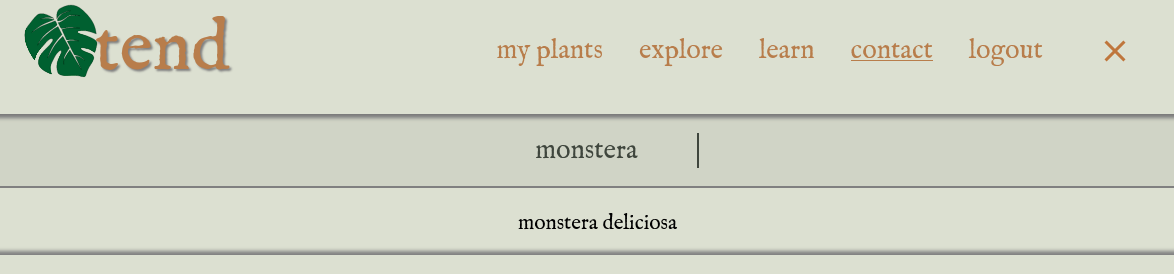
\includegraphics[width = 14cm]{search trim.png}
				\end{center}


	\section{Project}
	\subsection{What I accomplished this week}
	 	This week I have successfully added in both Vue Router and Vuex. Vue Router allowed me to use paths within the url to visit certain pages. Vuex is a central store that allows me to store the user login information (such as if a user is logged in and what their name is). I have also implemented the login page which allows the user to login to their account.\\

	 	For design, I have implemented more transitions throughout my application to make it more polished. Reflecting the purpose of the design, this softens the harsh default transitions, lining it up with my design purpose.\\

	 	Finally I have worked on deploying my app so far at tend.brandonmurch.com.\\

	\subsection{What I would like to accomplish next week}
		Next week I would like to create the MyPlants page, and necessary sub-pages. This will allow the user to view all their plants, upload new plants, view their notifications and change settings. This should take me roughly 8 hours to create a polished project.

\pagebreak
\end{document}